
\documentclass{article}

\usepackage[lofdepth,lotdepth]{subfig}

%
\usepackage{mathptmx}      % use Times fonts if available on your TeX system
%
% insert here the call for the packages your document requires
\usepackage{amssymb}
\usepackage{amsmath}
\usepackage{amsfonts}
\usepackage{epstopdf}
\usepackage{mathrsfs} % para formato de letra
\usepackage{hyperref}
\usepackage{enumitem}
\usepackage{array}
\usepackage{tabularx}
\usepackage{supertabular}
\usepackage{fancyhdr}
\usepackage{multirow}
\usepackage{color}
\usepackage{makeidx}
\usepackage{xstring}
\usepackage{setspace}
\usepackage{epsfig}

\usepackage{pgf}
% \usepgfplotslibrary{external} 
% \tikzexternalize

%\usepackage{subfigure}
\usepackage{preview}
% Packages to write pseudo-algorithms %
\usepackage{algorithm}
\usepackage{algorithmic}

% Tikz
\usepackage{stanli}
\usepackage[ugly]{units}
% \usetikzlibrary{decorations}
% \usetikzlibrary{arrows}
\usetikzlibrary{plotmarks}


\begin{document}

%%%%%%%%%%%%%%%%%%%%%%%%%%%%%%%%%%%%%%%%%%%%%%%%%%%%%%%%%%%%%%%%

\begin{figure}\sidecaption
  \centering
  \resizebox{0.9\hsize}{!}{
    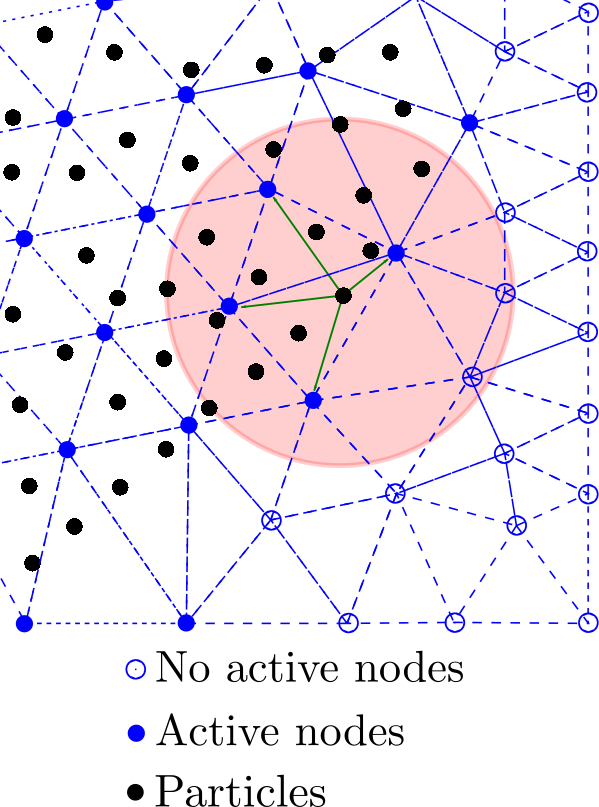
\includegraphics[width=\textwidth]{./Figures/Discretization_MPM}
  }
  \caption{Discretization used in the material point method.}
  \label{fig:MPM-discretization}
\end{figure}

%%%%%%%%%%%%%%%%%%%%%%%%%%%%%%%%%%%%%%%%%%%%%%%%%%%%%%%%%%%%%%%%

\begin{figure}\sidecaption
  \centering
  \resizebox{0.4\hsize}{!}{
    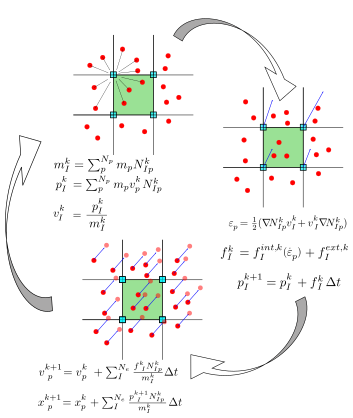
\includegraphics[width=\textwidth]{./Figures/MPM_scheme}
  }
  \caption{Classic material point method algorithm.}
  \label{fig:MPM_algorithm}
\end{figure}

%%%%%%%%%%%%%%%%%%%%%%%%%%%%%%%%%%%%%%%%%%%%%%%%%%%%%%%%%%%%%%%%

\begin{figure}
  \centering
  %%%%%%%%%%%%%%%%%%%%%%%%%%%%%%%%%%%%%%%%%%%%%% 
  \subfloat[Piecewise linear (Q4).]{
    \includegraphics[width=0.23\columnwidth]{Figures/MPM_Shape_Fun}
    \includegraphics[width=0.23\columnwidth]{Figures/MPM_Shape_Fun_dx}
    \includegraphics[width=0.23\columnwidth]{Figures/MPM_Shape_Fun_dy}
    \label{fig:MPM_Shape_Fun}
  }
  %%%%%%%%%%%%%%%%%%%%%%%%%%%%%%%%%%%%%%%%%%%%%% 
  \qquad
  %%%%%%%%%%%%%%%%%%%%%%%%%%%%%%%%%%%%%%%%%%%%%% 
  \subfloat[Local \textit{max-ent} $\gamma=17$.]{
    \includegraphics[width=0.23\columnwidth]{Figures/LME_17_3_Shape_Fun}
    \includegraphics[width=0.23\columnwidth]{Figures/LME_17_3_Shape_Fun_dx}
    \includegraphics[width=0.23\columnwidth]{Figures/LME_17_3_Shape_Fun_dy}
    \label{fig:LME_17.3_Shape_Fun}
  }
  %%%%%%%%%%%%%%%%%%%%%%%%%%%%%%%%%%%%%%%%%%%%%% 
  \qquad
  %%%%%%%%%%%%%%%%%%%%%%%%%%%%%%%%%%%%%%%%%%%%%% 
  \subfloat[Uniform GIMP (uGIMP).]{
    \includegraphics[width=0.23\columnwidth]{Figures/GIMP_Shape_Fun}
    \includegraphics[width=0.23\columnwidth]{Figures/GIMP_Shape_Fun_dx}
    \includegraphics[width=0.23\columnwidth]{Figures/GIMP_Shape_Fun_dy}
    \label{fig:GIMP_Shape_Fun}
  }
  %%%%%%%%%%%%%%%%%%%%%%%%%%%%%%%%%%%%%%%%%%%%%% 
  \qquad
  %%%%%%%%%%%%%%%%%%%%%%%%%%%%%%%%%%%%%%%%%%%%%%
  \subfloat[Local \textit{max-ent} $\gamma=10$.]{
    \includegraphics[width=0.23\columnwidth]{Figures/LME_10_0_Shape_Fun}
    \includegraphics[width=0.23\columnwidth]{Figures/LME_10_0_Shape_Fun_dx}
    \includegraphics[width=0.23\columnwidth]{Figures/LME_10_0_Shape_Fun_dy}
    \label{fig:LME_10.0_Shape_Fun}
  }
  %%%%%%%%%%%%%%%%%%%%%%%%%%%%%%%%%%%%%%%%%%%%%% 
  \qquad
  %%%%%%%%%%%%%%%%%%%%%%%%%%%%%%%%%%%%%%%%%%%%%%  
  \subfloat[Local \textit{max-ent} $\gamma=7$.]{
    \includegraphics[width=0.23\columnwidth]{Figures/LME_7_0_Shape_Fun}
    \includegraphics[width=0.23\columnwidth]{Figures/LME_7_0_Shape_Fun_dx}
    \includegraphics[width=0.23\columnwidth]{Figures/LME_7_0_Shape_Fun_dy}
    \label{fig:LME_7.0_Shape_Fun}
  }
  %%%%%%%%%%%%%%%%%%%%%%%%%%%%%%%%%%%%%%%%%%%%%% 
  \qquad
  %%%%%%%%%%%%%%%%%%%%%%%%%%%%%%%%%%%%%%%%%%%%%%  
  \subfloat[Local \textit{max-ent} $\gamma=5$.]{
    \includegraphics[width=0.23\columnwidth]{Figures/LME_5_0_Shape_Fun}
    \includegraphics[width=0.23\columnwidth]{Figures/LME_5_0_Shape_Fun_dx}
    \includegraphics[width=0.23\columnwidth]{Figures/LME_5_0_Shape_Fun_dy}
    \label{fig:LME_5.0_Shape_Fun}
  }
  \caption{Comparison of the local \textit{max-ent} shape function for
    different values of $\gamma = \beta h^2$, the piecewise linear shape function
    and the uniform GIMP shape function. The picture shows the nodal value
    of each shape function and its derivatives evaluated in a material
    point located in the center of the domain.}
  \label{fig:LME_MPM}
\end{figure}

%%%%%%%%%%%%%%%%%%%%%%%%%%%%%%%%%%%%%%%%%%%%%%%%%%%%%%%%%%%%%%%%

\begin{figure}\sidecaption
  \centering
  \resizebox{\hsize}{!}{
    \begin{tikzpicture} 
  \scaling{2}; 
  % Nodos 
  \point{a}{0}{1};
  \point{b}{3.75}{1};
  \point{c}{5}{1};
  % Barras
  \beam{2}{a}{b};
  \beam{2}{b}{c};
  % Apoyos
  \support{3}{a}[270];
  % Fuerzas
  \lineload{4}{b}{c}[1][0.2];
  \notation{5}{b}{c}[$5\ m/s$][.5][below][2];
  % Nombres de nodos
  \notation{1}{a}{A}[below right];
  \notation{1}{b}{B}[below right];
  \notation{1}{c}{C}[below right];
  % Cotas
  \dimensioning{1}{a}{b}{0.5}[{\unit[3/4]{L}}];
  \dimensioning{1}{b}{c}{0.5}[{\unit[1/4]{L}}];
\end{tikzpicture}
}
  \caption{Geometrical description of the Dyka \cite{Dyka1995} bar.}
  \label{fig:Dyka_Bar}
\end{figure}

\begin{figure}\sidecaption
  \centering
  \resizebox{\hsize}{!}{
    \includegraphics[width=\textwidth]{./Figures/Velocity_FE_vs_PCE_CFL_05}
  }
  \caption{Velocity evolution in the bar left side. This picture
    shows a comparison of both time integration algorithms,
    the Forward-Euler (FE) and the Predictor-Corrector explicit (PCE).}
  \label{fig:Velocity-Dyka-PCE-FE}
\end{figure}

\begin{figure}\sidecaption
  \centering
  \resizebox{\hsize}{!}{
    \includegraphics[width=\textwidth]{./Figures/Stress_FE_vs_PCE_CFL_05}
  }
  \caption{Stress evolution in the bar left side. This picture
    shows a comparison of both time integration algorithms,
    the Forward-Euler (FE) and the Predictor-Corrector explicit (PCE).}
  \label{fig:Stress-Dyka-PCE-FE}
\end{figure}

\begin{figure}\sidecaption
  \centering
  \resizebox{\hsize}{!}{    \includegraphics[width=\textwidth]{./Figures/Velocity_MPM_LME_gamma_comparative}
  }
  \caption{Velocity evolution at the point in the bar left side.}
  \label{fig:Velocity-Dyka-LME-gamma-comparative}
\end{figure}


\begin{figure}\sidecaption
  \centering
  \resizebox{\hsize}{!}{    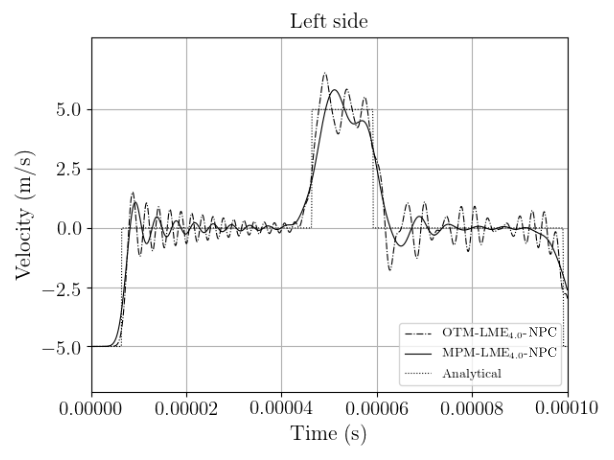
\includegraphics[width=\textwidth]{./Figures/Velocity_MPM_vs_OTM_Dyka}
  }
  \caption{Velocity evolution at the point in the bar left side.}
  \label{fig:Velocity-Dyka-MPM-vs-OTM}
\end{figure}


\begin{figure}\sidecaption
  \centering
  \resizebox{\hsize}{!}{    \includegraphics[width=\textwidth]{./Figures/Velocity_Q4_vs_uGIMP_LME_Dyka}
  }
  \caption{Velocity evolution at the point in the bar left side.}
  \label{fig:Velocity-Dyka-Q4-uGIMP-LME}
\end{figure}

%%%%%%%%%%%%%%%%%%%%%%%%%%%%%%%%%%%%%%%%%%%%%%%%%%%%%%%%%%%%%%%%

\begin{figure}\sidecaption
  \centering
  \resizebox{\hsize}{!}{
    \begin{tikzpicture} 
  \scaling{1};
  
% Nodos
\point{1}{0}{10};
\point{2}{2}{10};
\point{3}{0}{8};
\point{4}{2}{8};
\point{5}{4}{10};
\point{6}{0}{6};
\point{7}{2}{6};
\point{8}{4}{8};
\point{9}{4}{6};
\point{10}{6}{10};
\point{11}{0}{4};            
\point{12}{2}{4};            
\point{13}{6}{8};            
\point{14}{4}{4};            
\point{15}{6}{6};            
\point{16}{8}{10};            
\point{17}{0}{2};            
\point{18}{2}{2};            
\point{19}{8}{8};            
\point{20}{6}{4};            
\point{21}{4}{2};            
\point{22}{8}{6};            
\point{23}{0}{0};            
\point{24}{10}{10};            
\point{25}{6}{2};            
\point{26}{8}{4};
\point{27}{2}{0};            
\point{28}{10}{8};            
\point{29}{4}{0};            
\point{30}{10}{6};            
\point{31}{8}{2};            
\point{32}{6}{0};            
\point{33}{10}{4};            
\point{34}{8}{0};            
\point{35}{10}{2};            
\point{36}{10}{0};

% Barras
\beam{2}{27}{18};
\beam{2}{18}{17};
\beam{2}{17}{23};
\beam{2}{23}{27};
  
\beam{2}{29}{21};
\beam{2}{21}{18};
\beam{2}{18}{27};
\beam{2}{29}{27};

\beam{2}{32}{25};
\beam{2}{25}{21};
\beam{2}{21}{29};
\beam{2}{32}{29};

\beam{2}{34}{31};
\beam{2}{31}{25};
\beam{2}{25}{32};
\beam{2}{34}{32};

\beam{2}{36}{35};
\beam{2}{35}{31};
\beam{2}{31}{34};
\beam{2}{36}{34};

%%%%%%%%%%%%%%%%
\beam{2}{18}{12};
\beam{2}{12}{11};
\beam{2}{11}{17};
\beam{2}{18}{17};

\beam{2}{21}{14};
\beam{2}{14}{12};
\beam{2}{12}{18};
\beam{2}{21}{18};

\beam{2}{25}{20};
\beam{2}{20}{14};
\beam{2}{14}{21};
\beam{2}{25}{21};

\beam{2}{31}{26};
\beam{2}{26}{20};
\beam{2}{20}{25};
\beam{2}{31}{25};

\beam{2}{35}{33};
\beam{2}{33}{26};
\beam{2}{26}{31};
\beam{2}{35}{31};

%%%%%%%%%%%%%%%%
\beam{2}{12}{7};
\beam{2}{7}{6};
\beam{2}{6}{11};
\beam{2}{12}{11};

\beam{2}{14}{9};
\beam{2}{9}{7};
\beam{2}{7}{12};
\beam{2}{14}{12};

\beam{2}{20}{15};
\beam{2}{15}{9};
\beam{2}{9}{14};
\beam{2}{20}{14};

\beam{2}{26}{22};
\beam{2}{22}{15};
\beam{2}{15}{20};
\beam{2}{26}{20};

\beam{2}{33}{30};
\beam{2}{30}{22};
\beam{2}{22}{26};
\beam{2}{33}{26};

%%%%%%%%%%%%%%%%
\beam{2}{7}{4};
\beam{2}{4}{3};
\beam{2}{3}{6};
\beam{2}{7}{6};

\beam{2}{9}{8};
\beam{2}{8}{4};
\beam{2}{4}{7};
\beam{2}{9}{7};

\beam{2}{15}{13};
\beam{2}{13}{8};
\beam{2}{8}{9};
\beam{2}{15}{9};

\beam{2}{22}{19};
\beam{2}{19}{13};
\beam{2}{13}{15};
\beam{2}{22}{15};

\beam{2}{30}{28};
\beam{2}{28}{19};
\beam{2}{19}{22};
\beam{2}{30}{22};

%%%%%%%%%%%%%%%%
\beam{2}{4}{2};
\beam{2}{2}{1};
\beam{2}{1}{3};
\beam{2}{4}{3};

\beam{2}{8}{5};
\beam{2}{5}{2};
\beam{2}{2}{4};
\beam{2}{8}{4};

\beam{2}{13}{10};
\beam{2}{10}{5};
\beam{2}{5}{8};
\beam{2}{13}{8};

\beam{2}{19}{16};
\beam{2}{16}{10};
\beam{2}{10}{13};
\beam{2}{19}{13};

\beam{2}{28}{24};
\beam{2}{24}{16};
\beam{2}{16}{19};
\beam{2}{28}{19};

% Bottom
\support {1}{23}[315];
\support {1}{27}[0];
\support {1}{29}[0];
\support {1}{32}[0];
\support {1}{34}[0];
\support {1}{36}[45];

% \support {2}{23}[270];
\support {2}{1}[270];
\support {2}{3}[270];
\support {2}{6}[270];
\support {2}{11}[270];
\support {2}{17}[270];

\support {2}{24}[90];
\support {2}{28}[90];
\support {2}{30}[90];
\support {2}{33}[90];
\support {2}{35}[90];
% \support {2}{36}[90];

% Gravity
\point{g}{12}{5};
\load{1}{g}[90][3][0];

% Cotas
\dimensioning{1}{23}{36}{-1.5}[$10~m$];
\dimensioning{2}{23}{1}{-1.5}[$10~m$];


\end{tikzpicture}


% % Apoyos
% \support{3}{c}[90];
% % Fuerzas
% \lineload{4}{b}{a}[1][0.2];
% \notation{5}{a}{b}[$-5\ m/s$][.5][below][2];
% % Nombres de nodos
% \notation{1}{a}{A}[below left];
% \notation{1}{b}{B}[below left];
% \notation{1}{c}{C}[below left];
% % Cotas
% \dimensioning{1}{a}{b}{0.5}[{\unit[1/4]{L}}];
% \dimensioning{1}{b}{c}{0.5}[{\unit[3/4]{L}}];


% End Elements
}
  \caption{Geometrical description of a soil block }.}
  \label{fig:block}
\end{figure}


\begin{figure}\sidecaption
  \centering
  \resizebox{\hsize}{!}{
    \includegraphics[width=\textwidth]{./Figures/Block_CFL_01_Comparative}
  }
  \caption{Comparative of the vertical displacement evolution in a
    point located in the free surface employing different
    interpolation schemes and numerical techniques.} 
  \label{fig:vertical-displacement-block}
\end{figure}

\begin{figure}
  \centering
  %%%%%%%%%%%%%%%%%%%%%%%%%%%%%%%%%%%%%%%%%%%%%% 
  \subfloat[t = 0 seconds.]{
    \includegraphics[width=0.5\columnwidth]{Figures/Block_LME3_PCE_a_t0}
    \label{fig:Block-LME3-PCE-t0}
  }
  %%%%%%%%%%%%%%%%%%%%%%%%%%%%%%%%%%%%%%%%%%%%%% 
  \qquad
  %%%%%%%%%%%%%%%%%%%%%%%%%%%%%%%%%%%%%%%%%%%%%% 
  \subfloat[t = 5 seconds.]{
    \includegraphics[width=0.5\columnwidth]{Figures/Block_LME3_PCE_b_t025}
    \label{fig:Block-LME3-PCE-t025}
  }
  %%%%%%%%%%%%%%%%%%%%%%%%%%%%%%%%%%%%%%%%%%%%%%
  \qquad
  %%%%%%%%%%%%%%%%%%%%%%%%%%%%%%%%%%%%%%%%%%%%%% 
  \subfloat[t = 20 seconds]{
    \includegraphics[width=0.5\columnwidth]{Figures/Block_LME3_PCE_c_t1}
    \label{fig:Block-LME3-PCE-t1}
  }
  %%%%%%%%%%%%%%%%%%%%%%%%%%%%%%%%%%%%%%%%%%%%%% 
  \caption{Vertical normal stress and position of material points
    during the loading process for a soft soil ($E = 5\ MPa$, $\rho_0
    = 6\cdot 10^3\ kg/m^3$). Numerical parameters considered for the
    simulation are : Local \textit{max-ent} shape function $\gamma =3$
    and explicit PC scheme with CFL 0.1.}
  \label{fig:Block-LME3}
\end{figure}

%%%%%%%%%%%%%%%%%%%%%%%%%%%%%%%%%%%%%%%%%%%%%%%%%%%%%%%%%%%%%%%%

\begin{figure}\sidecaption
  \centering
  \resizebox{\hsize}{!}{
    \includegraphics[width=\columnwidth]{Figures/1D_right_Velocity.png}
  }
  \caption[Velocities values in the right side of the Dyka
  bar]{Analytical solution for the velocity in the right side of the Dyka bar.}
  \label{fig:vel_analytics_dyka}
\end{figure}

\begin{figure}\sidecaption
  \centering
  \resizebox{\hsize}{!}{
    \includegraphics[width=\columnwidth]{Figures/1D_left_Stress.png}
  }
  \caption[Stress values in the last quarter side of the Dyka
  bar]{Analytical solution for the stress in the last quarter of the Dyka bar.}
  \label{fig:stress_analytics_dyka}
\end{figure}


\end{document}



